%%%%%%%%%%%%%%%%%%%%%%%%%%%%%%%%%%%%%%%%%
% Structured General Purpose Assignment
% LaTeX Template
%
% This template has been downloaded from:
% http://www.latextemplates.com
%
% Original author:
% Ted Pavlic (http://www.tedpavlic.com)
%
% Note:
% The \lipsum[#] commands throughout this template generate dummy text
% to fill the template out. These commands should all be removed when 
% writing assignment content.
%
%%%%%%%%%%%%%%%%%%%%%%%%%%%%%%%%%%%%%%%%%

%----------------------------------------------------------------------------------------
%	PACKAGES AND OTHER DOCUMENT CONFIGURATIONS
%----------------------------------------------------------------------------------------

\documentclass{article}

\usepackage{listings}
\usepackage{mathtools}
\usepackage{fancyhdr} % Required for custom headers
\usepackage{lastpage} % Required to determine the last page for the footer
\usepackage{extramarks} % Required for headers and footers
\usepackage{graphicx} % Required to insert images
\usepackage{lipsum} % Used for inserting dummy 'Lorem ipsum' text into the template
\usepackage{caption}
\usepackage{subcaption}
\usepackage{amsmath}

% Margins
\topmargin=-0.45in
\evensidemargin=0in
\oddsidemargin=0in
\textwidth=6.5in
\textheight=9.0in
\headsep=0.25in 

\linespread{1.1} % Line spacing

% Set up the header and footer
\pagestyle{fancy}
\lhead{\hmwkAuthorName} % Top left header
\chead{\hmwkClass} % Top center header   -->  \ (\hmwkClassInstructor\ \hmwkClassTime): \hmwkTitle
\rhead{\firstxmark} % Top right header
\lfoot{\lastxmark} % Bottom left footer
\cfoot{} % Bottom center footer
\rfoot{Page\ \thepage\ of\ \pageref{LastPage}} % Bottom right footer
\renewcommand\headrulewidth{0.4pt} % Size of the header rule
\renewcommand\footrulewidth{0.4pt} % Size of the footer rule

\setlength\parindent{0pt} % Removes all indentation from paragraphs

%----------------------------------------------------------------------------------------
%	DOCUMENT STRUCTURE COMMANDS
%	Skip this unless you know what you're doing
%----------------------------------------------------------------------------------------

% Header and footer for when a page split occurs within a problem environment
\newcommand{\enterProblemHeader}[1]{
\nobreak\extramarks{#1}{#1 continued on next page\ldots}\nobreak
\nobreak\extramarks{#1 (continued)}{#1 continued on next page\ldots}\nobreak
}

% Header and footer for when a page split occurs between problem environments
\newcommand{\exitProblemHeader}[1]{
\nobreak\extramarks{#1 (continued)}{#1 continued on next page\ldots}\nobreak
\nobreak\extramarks{#1}{}\nobreak
}

\setcounter{secnumdepth}{0} % Removes default section numbers
\newcounter{homeworkProblemCounter} % Creates a counter to keep track of the number of problems

\newcommand{\homeworkProblemName}{}
\newenvironment{homeworkProblem}[1][Problem \arabic{homeworkProblemCounter}]{ % Makes a new environment called homeworkProblem which takes 1 argument (custom name) but the default is "Problem #"
\stepcounter{homeworkProblemCounter} % Increase counter for number of problems
\renewcommand{\homeworkProblemName}{#1} % Assign \homeworkProblemName the name of the problem
\section{\homeworkProblemName} % Make a section in the document with the custom problem count
\enterProblemHeader{\homeworkProblemName} % Header and footer within the environment
}{
\exitProblemHeader{\homeworkProblemName} % Header and footer after the environment
}

\newcommand{\problemAnswer}[1]{ % Defines the problem answer command with the content as the only argument
\noindent\framebox[\columnwidth][c]{\begin{minipage}{0.98\columnwidth}#1\end{minipage}} % Makes the box around the problem answer and puts the content inside
}

\newcommand{\homeworkSectionName}{}
\newenvironment{homeworkSection}[1]{ % New environment for sections within homework problems, takes 1 argument - the name of the section
\renewcommand{\homeworkSectionName}{#1} % Assign \homeworkSectionName to the name of the section from the environment argument
\subsection{\homeworkSectionName} % Make a subsection with the custom name of the subsection
\enterProblemHeader{\homeworkProblemName\ [\homeworkSectionName]} % Header and footer within the environment
}{
\enterProblemHeader{\homeworkProblemName} % Header and footer after the environment
}
   
%----------------------------------------------------------------------------------------
%	NAME AND CLASS SECTION
%----------------------------------------------------------------------------------------

\newcommand{\hmwkTitle}{Project\ \#2} % Assignment title
\newcommand{\hmwkDueDate}{Wednesday,\ March\ 4,\ 2015} % Due date
\newcommand{\hmwkClass}{CSCI\ 8810} % Course/class
\newcommand{\hmwkClassTime}{08:00am} % Class/lecture time
\newcommand{\hmwkClassInstructor}{Prof. Arabnia} % Teacher/lecturer
\newcommand{\hmwkAuthorName}{Sina Solaimanpour} % Your name

%----------------------------------------------------------------------------------------
%	TITLE PAGE
%----------------------------------------------------------------------------------------

\title{
\vspace{2in}
\textmd{\textbf{\hmwkClass:\ \hmwkTitle}}\\
\normalsize\vspace{0.1in}\small{Due\ on\ \hmwkDueDate}\\
\vspace{0.1in}\large{\textit{\hmwkClassInstructor\ \hmwkClassTime}}
\vspace{3in}
}

\author{\textbf{\hmwkAuthorName}}
\date{} % Insert date here if you want it to appear below your name

%----------------------------------------------------------------------------------------

\begin{document}

\maketitle

%----------------------------------------------------------------------------------------
%	TABLE OF CONTENTS
%----------------------------------------------------------------------------------------

%\setcounter{tocdepth}{1} % Uncomment this line if you don't want subsections listed in the ToC

\newpage
\tableofcontents
\newpage

%----------------------------------------------------------------------------------------
%	Introduction
%----------------------------------------------------------------------------------------

% To have just one problem per page, simply put a \clearpage after each problem

\begin{homeworkProblem}[\Roman{homeworkProblemCounter}. Introduction]
In this paper, I will discuss about the second phase of the ColonD Image processing project. The first phase of the project was about designing the overall structure of the project and implement some basic operations like read/write, gray-scale conversion, thresholding and smoothing images by applying filters. In this phase of the of the project, I will expand the program to include some other filtering operations and another slightly more complicated feature called Connected Components Labelling or CCL.


The following list shows what new features have been added to the program in phase 2:
\begin{itemize} \itemsep1pt \parskip0pt \parsep0pt
  \item Connected Component Labelling (CCL)
  \item Invert pixel colors
  \item Robert's operator
  \item Sobel's operator
  \item Prewitt's operator
  \item Kirsch's operator
  \item Laplacian filter
  \item Gaussian filter
\end{itemize}

These features are all implemented and tested with different images, individually and in combination of other operations. In the next sections, I will go over each one of these features in more detail and will present some results from the program.
\end{homeworkProblem}

%----------------------------------------------------------------------------------------
%	Component Labelling
%----------------------------------------------------------------------------------------

% To have just one problem per page, simply put a \clearpage after each problem

\begin{homeworkProblem}[\Roman{homeworkProblemCounter}. Connected Component Labelling]
Connected Component Labelling is a well-known algorithm used to find individual components in an image. The idea behind this version of the algorithm is to check the surrounding pixels (in this case, the west and the north pixels) of a white pixel and assign appropriate label to the pixel in hand. Details of this pixel are as follows:
\begin{enumerate} \itemsep1pt \parskip0pt \parsep0pt
  \item If the north and west pixels are black: Assign a new label to the pixel
  \item If west pixel is white and the other one is black: Assign the label of the west pixel to the pixel in hand
  \item If north pixel is white and the other one is black: Assign the label of the north pixel to the pixel in hand
  \item If both west and north pixels are white: Assign to the pixel in hand, the smaller label of the two and record that the two labels are equivalent.
\end{enumerate}

The algorithm described above is the first pass of the CCL algorithm. After labelling each pixel during the first pass, we need to go over all of the pixels and handle the equivalent labels found in the first pass. As the number of labels during the first pass might get very big, I am using a \textbf{Disjoint Set Data Structure}  implemented in \textbf{Boost framework}. The overall idea of the disjoint set dadta structure is to keep the equivalent elements as a set represented by the smallest member of that set. When a new label is created, it is considered to be a separate set in the bigger set. Later on in the program, when an equivalency is found between two labels, the sets representing those two labels are merged together with a union function. This will allow us to know exactly which labels are equivalent with each other. 

During the second pass, we find the set that each label is a member of and use the representing label in that set as the final label.

Just for better visualization of the components, I use a very simple coloring technique which might fail from time to time, depending on the number of the components found and their order, but it will try to assign distinct colors to different components found in the image.

Figure \ref{fig:CCL1} shows the process of labelling the lena's image. First the image is converted to gray scale. Then, I apply some gaussian smoothing to the image and use the simple thresholding feature to convert the image to a binary image with some disjoint components. At the end, I use the CCL in the program to label the components in the resulting image from the previous steps.

\begin{figure}[h!]
  \centering
	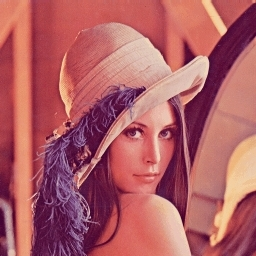
\includegraphics[width=0.3\textwidth]{CCL1-1}
	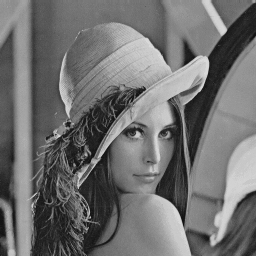
\includegraphics[width=0.3\textwidth]{CCL1-2}
	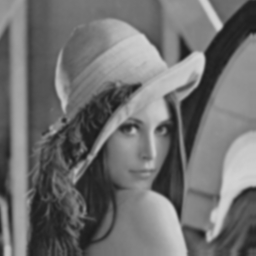
\includegraphics[width=0.3\textwidth]{CCL1-3}
	
\includegraphics[width=0.3\textwidth]{CCL1-4}
	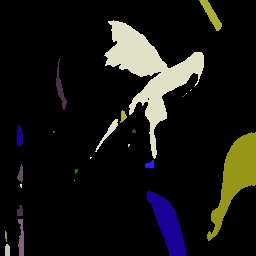
\includegraphics[width=0.3\textwidth]{CCL1-5}
  \caption{The resulting images from using the CCL algorithm on the lena's image after applying a gray-scale conversion, two gaussian filters and a simple thresholding. Different colors in the last image shows different components found. Here, we have \textbf{29} distinct components with average component area of \textbf{300.276} pixels.}
  \label{fig:CCL1}
\end{figure}

In the next example, shown in Figure \ref{fig:CCL2}, I have tried to show that CCL can be used to find important parts of an image of a human face. The image used in this example was obtained randomly from a search for "Face Image" on Google and was in gray-scale originally. Two Guassian filters have been applied to the image and after that, the image has been converted to binary using a thresholding technique. CCL has been used on the image after inverting the image pixels. The result is very interesting because you can clearly see that the important parts of the face (her eyes, lib, nose and a not very complete boundary around the face) have been highlighted as different components.

\begin{figure}[h!]
  \centering
	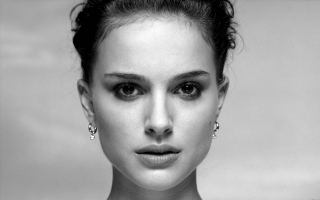
\includegraphics[width=0.3\textwidth]{CCL2-1}
	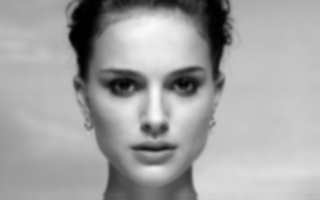
\includegraphics[width=0.3\textwidth]{CCL2-2}
	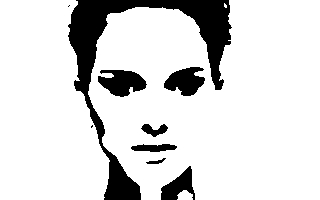
\includegraphics[width=0.3\textwidth]{CCL2-3}
	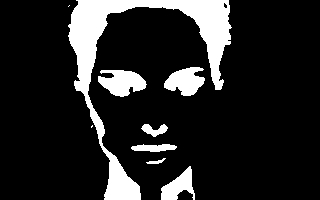
\includegraphics[width=0.3\textwidth]{CCL2-4}
	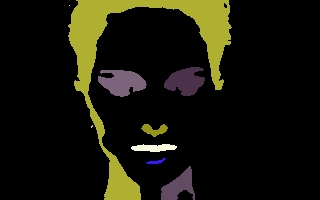
\includegraphics[width=0.3\textwidth]{CCL2-5}
  \caption{Applying CCL to an image of a face. Different colors in the last image shows different components found. Here, we have \textbf{10} distinct components with average component area of \textbf{926} pixels.}
  \label{fig:CCL2}
\end{figure}

\end{homeworkProblem}

%----------------------------------------------------------------------------------------
%	Invert
%----------------------------------------------------------------------------------------

% To have just one problem per page, simply put a \clearpage after each problem

\begin{homeworkProblem}[\Roman{homeworkProblemCounter}. Invert]

Inverting an image has been implemented in the program as an extra feature. It will subtract the pixel value from 255 and use the resulting value as the pixel intensity. This function is illustrated in Figure \ref{fig:invert}.

\begin{figure}[h!]
  \centering
	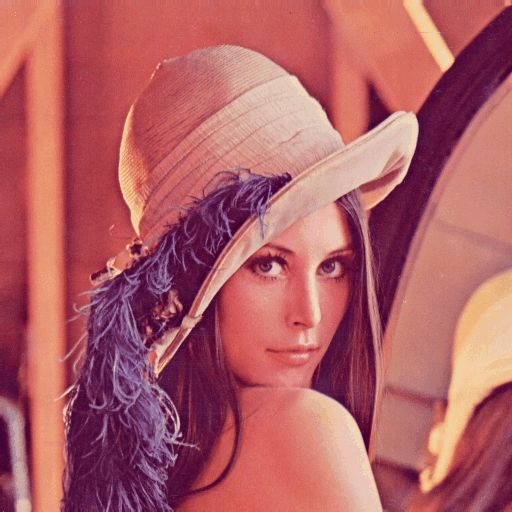
\includegraphics[width=0.3\textwidth]{invert1}
	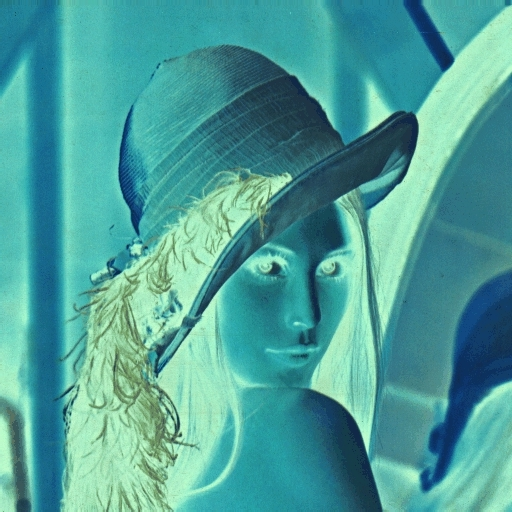
\includegraphics[width=0.3\textwidth]{invert2}
  \caption{Inverting pixel values of the lena's image.}
  \label{fig:invert}
\end{figure}

\end{homeworkProblem}

%----------------------------------------------------------------------------------------
%	Robert's operator
%----------------------------------------------------------------------------------------

% To have just one problem per page, simply put a \clearpage after each problem

\begin{homeworkProblem}[\Roman{homeworkProblemCounter}. Robert's Operator]
Robert's operator is acting as an edge detector. The operator is consisting of separate applications of two different 2 x 2 filters. The idea behind this operator is to approximate the gradient of an image. The matrices used as filters are shown below.
\[
F1 =\begin{bmatrix}
    +1 & 0 \\
    0 & -1
\end{bmatrix}
,
F2 =\begin{bmatrix}
	0 & +1 \\
	-1 & 0
\end{bmatrix}
\]

These two filters are applied to the image individually and at the end, the final result would be the summation of both images together. I will present two examples of this operator used on different images.

The first application of the operator was on an image of a bike in front of a brick wall. The operator is applied without any other modifications to the image and the result is shown in Figure \ref{fig:rob1}.

\begin{figure}[h!]
  \centering
	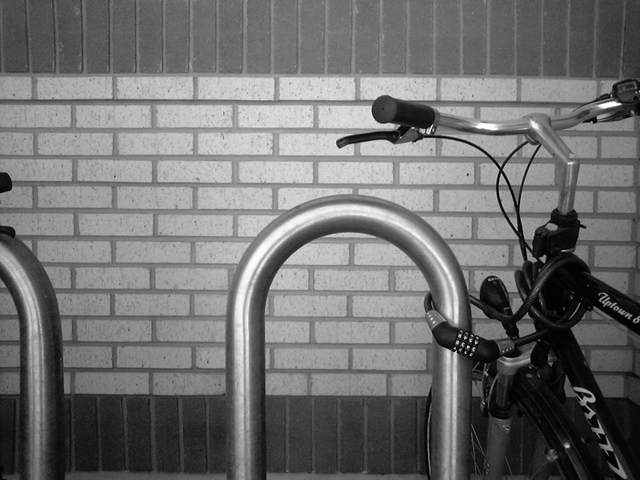
\includegraphics[width=0.3\textwidth]{rob1-1}
	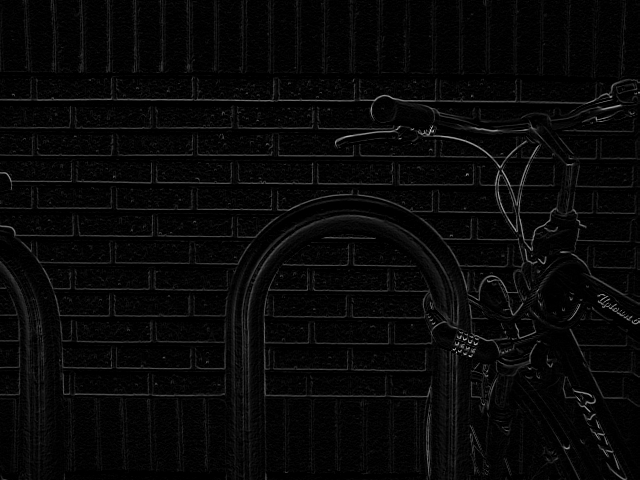
\includegraphics[width=0.3\textwidth]{rob1-2}
  \caption{Applying Robert's operator to an image without any other modifications.}
  \label{fig:rob1}
\end{figure}

Now, I am going to show the resulting image from Robert's operator to the same image but with applying a Guassian filter before the Robert's application. The results are shown in Figure \ref{fig:rob2}.

\begin{figure}[h!]
  \centering
	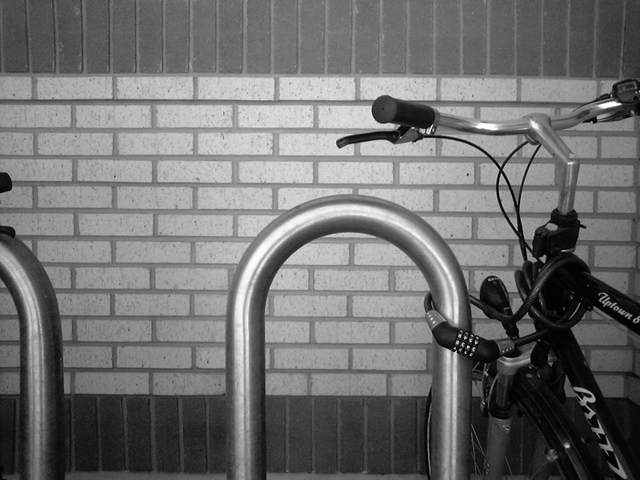
\includegraphics[width=0.3\textwidth]{rob2-1}
	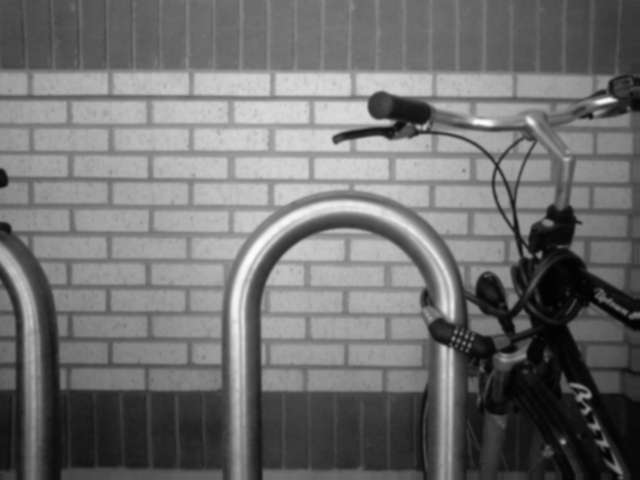
\includegraphics[width=0.3\textwidth]{rob2-2}
	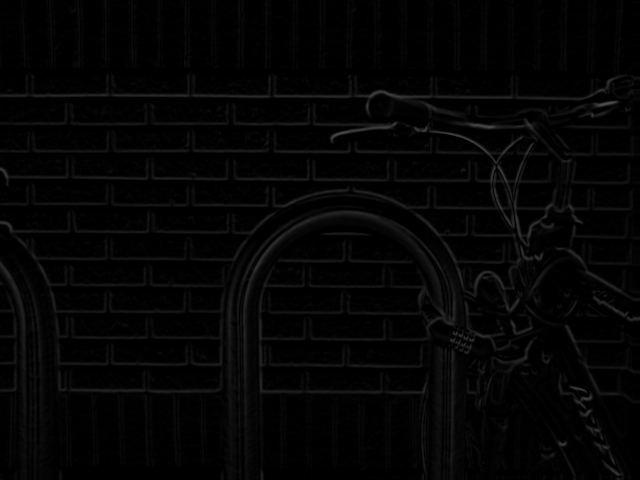
\includegraphics[width=0.3\textwidth]{rob2-3}
  \caption{Applying Robert's operator to an image with Guassian filter applied to it.}
  \label{fig:rob2}
\end{figure}

As you can see, the difference between the results of the Robert's operator to an image with or without the Guassian filter is not big. Although, if you pay attention closer, the difference is in the amount of noise shown in two results. The image with Guassian filter applied to it, has much smoother surface which allows us to focus on the important information not getting confused with the noise.

\end{homeworkProblem}

%----------------------------------------------------------------------------------------
%	Sobel's operator
%----------------------------------------------------------------------------------------

% To have just one problem per page, simply put a \clearpage after each problem

\begin{homeworkProblem}[\Roman{homeworkProblemCounter}. Sobel's Operator]
Sobel's operator is another edge detector. The operator is consisting of separate applications of two different 3 x 3 filters. The idea behind this operator is to use two filters, one focusing on Horizontal edges and the other one focused on the Vertical edges to find all of the edges in the image. The filters used in this operator is as follows:
\[
GY =\begin{bmatrix}
    -1 & -2 & -1 \\
    0 & 0 & 0 \\
    1 & 2 & 1 
\end{bmatrix}
,
GX =\begin{bmatrix}
    -1 & 0 & 1 \\
    -2 & 0 & 2 \\
    -1 & 0 & 1 
\end{bmatrix}
\]

These two filters are applied to the image individually and at the end, the final result would be the summation of both images together. I will present two examples of this operator used on different images.

The first application of the operator is on the same image used in the Robert's operator section (The bike's image). The operator is applied without any other modifications to the image and the result is shown in Figure \ref{fig:sob1}. As you can see, the edges are much brighter and stronger comparing to the edges found using Robert's operator.

\begin{figure}[h!]
  \centering
	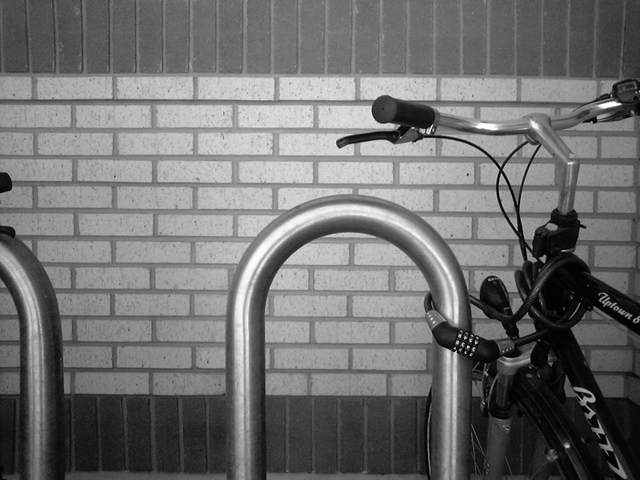
\includegraphics[width=0.3\textwidth]{sob1-1}
	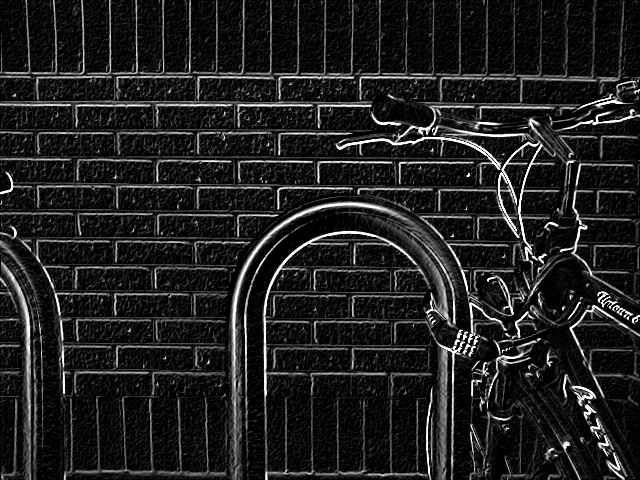
\includegraphics[width=0.3\textwidth]{sob1-2}
  \caption{Applying Sobel's operator to an image without any other modifications.}
  \label{fig:sob1}
\end{figure}

The second example of the Sobel's operator will be on the face image used in the previous sections. This is to illustrate how an edge detection algorithm will perform on an image which contains a face in it. The results can be seen in Figure \ref{fig:sob2}. The face image is first smoothed with an application of a Guassian filter. The result of this operator clearly shows that the important areas of the image are again highlighted and the main purpose of edge detection algorithms are to find and highlight important parts of the images which are the boundaries between different colors in the image.

\begin{figure}[h!]
  \centering
	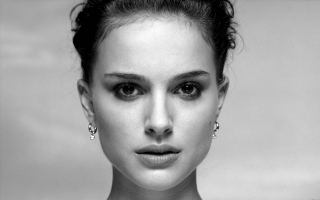
\includegraphics[width=0.3\textwidth]{sob2-1}
	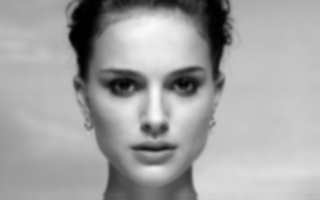
\includegraphics[width=0.3\textwidth]{sob2-2}
	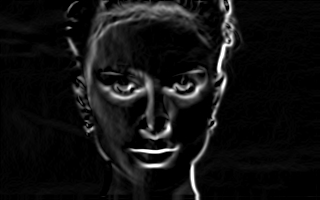
\includegraphics[width=0.3\textwidth]{sob2-3}
  \caption{Applying Sobel's operator to a face image with Guassian filter applied to it.}
  \label{fig:sob2}
\end{figure}

\end{homeworkProblem}

%----------------------------------------------------------------------------------------
%	Prewitt's operator
%----------------------------------------------------------------------------------------

% To have just one problem per page, simply put a \clearpage after each problem

\begin{homeworkProblem}[\Roman{homeworkProblemCounter}. Prewitt's Operator]
Prewitt's operator is again another edge detector operator like the previous two operators. The operator is consisting of separate applications of two different 3 x 3 filters. The idea behind this operator is very similar to the idea used in Sobel's operator which uses two filters, one focusing on Horizontal edges and the other one focused on the Vertical edges to find all of the edges in the image. The filters used in this operator is as follows:
\[
GY =\begin{bmatrix}
    -1 & -1 & -1 \\
    0 & 0 & 0 \\
    1 & 1 & 1 
\end{bmatrix}
,
GX =\begin{bmatrix}
    -1 & 0 & 1 \\
    -1 & 0 & 1 \\
    -1 & 0 & 1 
\end{bmatrix}
\]

These two filters are applied to the image individually and at the end, the final result would be the summation of both images together. Figure \ref{fig:prew1} depicts how this operator performs on the image of the bike used in previous sections. The result is very similar to the result of the Sobel's operator, but it can argued that the result of the Prewitt's operator is less biased towards the pixels in the middle of the filter.

\begin{figure}[h!]
  \centering
	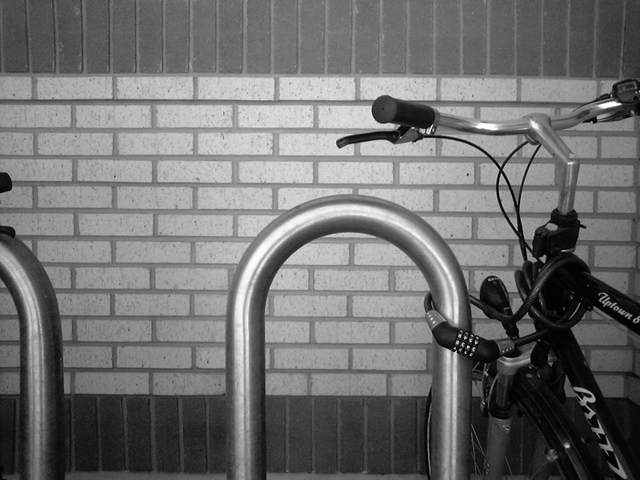
\includegraphics[width=0.3\textwidth]{prew1}
	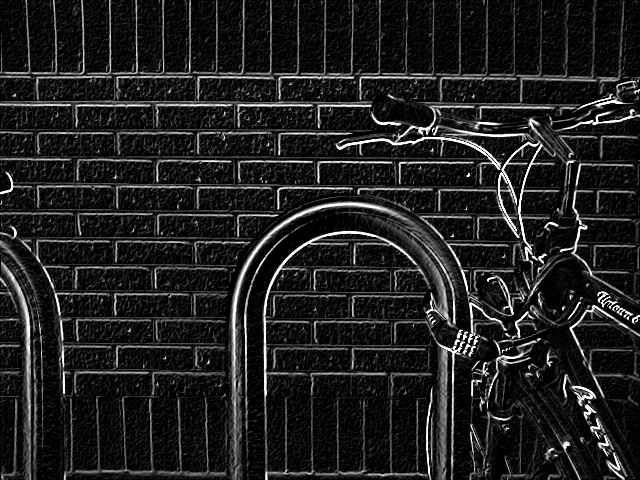
\includegraphics[width=0.3\textwidth]{prew2}
  \caption{Applying Prewitt's operator to an image without any other modifications.}
  \label{fig:prew1}
\end{figure}

\end{homeworkProblem}

%----------------------------------------------------------------------------------------
%	Kirsch's operator
%----------------------------------------------------------------------------------------

% To have just one problem per page, simply put a \clearpage after each problem

\begin{homeworkProblem}[\Roman{homeworkProblemCounter}. Kirsch's Operator]
Kirsch's operator is another edge detector operator but it acts a little bit differently than the others. The operator is consisting of separate applications of four different 3 x 3 filters. Two of the filters are biased towards the Horizontal and Vertical edges and the other two are simply a 45 degree rotation of these filters. The filters are as follow:
\[
F1 =\begin{bmatrix}
    1 & 1 & 1 \\
    0 & 0 & 0 \\
    -1 & -1 & -1 
\end{bmatrix}
,
F2 =\begin{bmatrix}
    -1 & 0 & 1 \\
    -1 & 0 & 1 \\
    -1 & 0 & 1 
\end{bmatrix}
,
F3 =\begin{bmatrix}
    0 & 1 & 1 \\
    -1 & 0 & 1 \\
    -1 & -1 & 0 
\end{bmatrix}
,
F4 =\begin{bmatrix}
    1 & 1 & 0 \\
    1 & 0 & -1 \\
    0 & -1 & -1 
\end{bmatrix}
\]

These filters are applied to the image individually and at the end, to combine the results, I find the maximum for each pixel among four pixels of the images and use that value to represent the final pixel value. Beside combining the resulting images from the four filters, I give the user the option to save all separate and the combined images to the file system. Figure \ref{fig:kirs1} depicts how this operator performs on the image of the bike used in previous sections by showing all four separate images and the combined result at the end. You can obviously see specially in the first two filtered images that the filter are working in favor of the Horizintal and Vertical edges, respectively. The other two filtered images are showing the results for the rotated filters and the last image shows the combined image using the max operator.

\begin{figure}[h!]
  \centering
	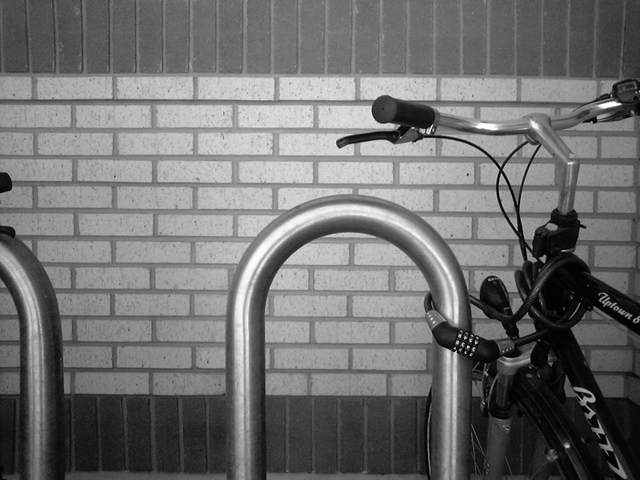
\includegraphics[width=0.3\textwidth]{kirs1-1}
	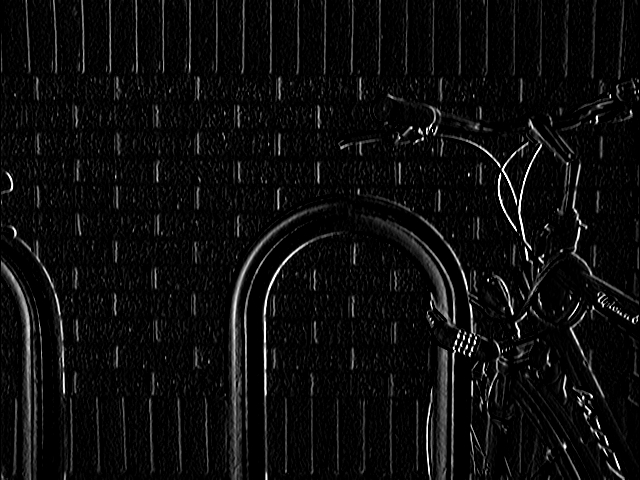
\includegraphics[width=0.3\textwidth]{kirs1-2}
	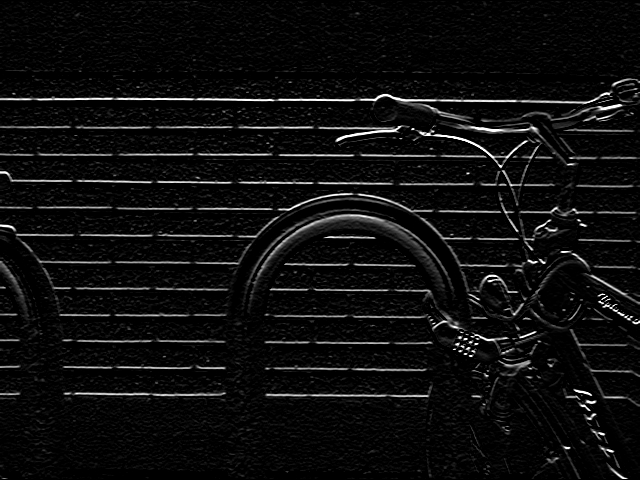
\includegraphics[width=0.3\textwidth]{kirs1-3}
	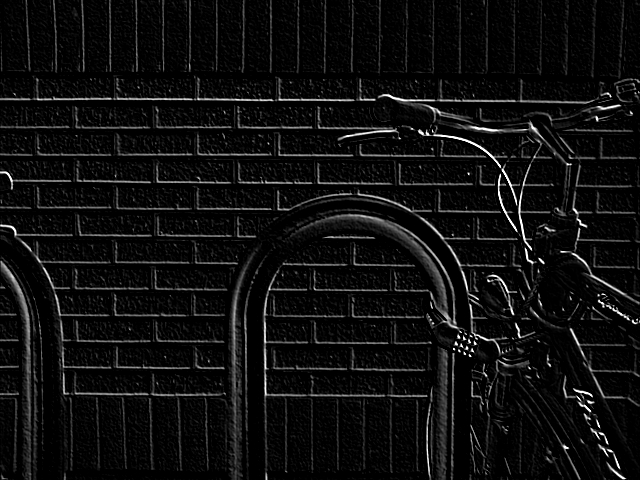
\includegraphics[width=0.3\textwidth]{kirs1-4}
	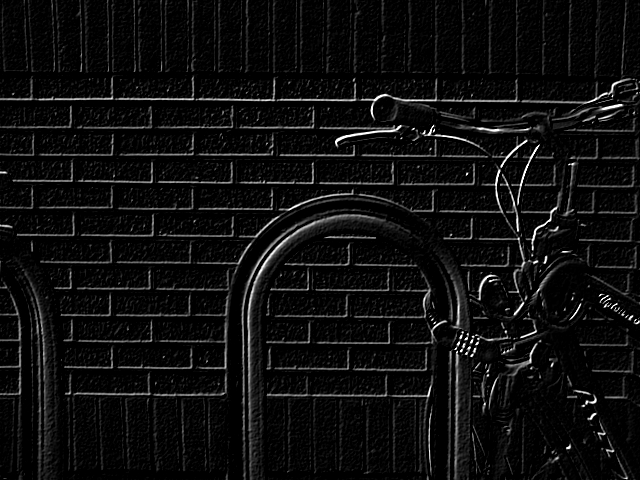
\includegraphics[width=0.3\textwidth]{kirs1-5}
	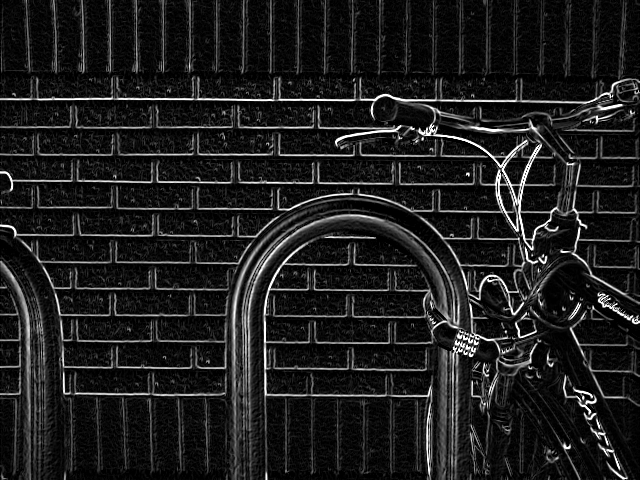
\includegraphics[width=0.3\textwidth]{kirs1-6}
  \caption{Applying Kirsch's operator to an image without any other modifications.}
  \label{fig:kirs1}
\end{figure}

Figure \ref{fig:kirs2} shows the usage of the Kirsch's operator on Lena's image. Again, all 4 separate and the combined images are shown in this figure. If one pay attention to the third and the fourth images, he can clearly see that these images are the results from the rotated filters because the edges with 45 degree headings are highlighted much stronger than other edges.

\begin{figure}[h!]
  \centering
	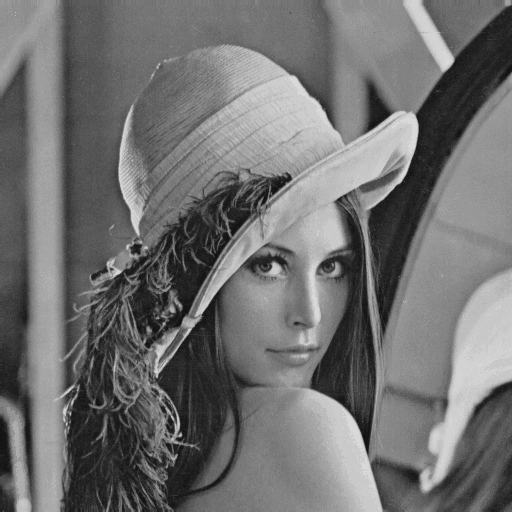
\includegraphics[width=0.3\textwidth]{kirs2-1}
	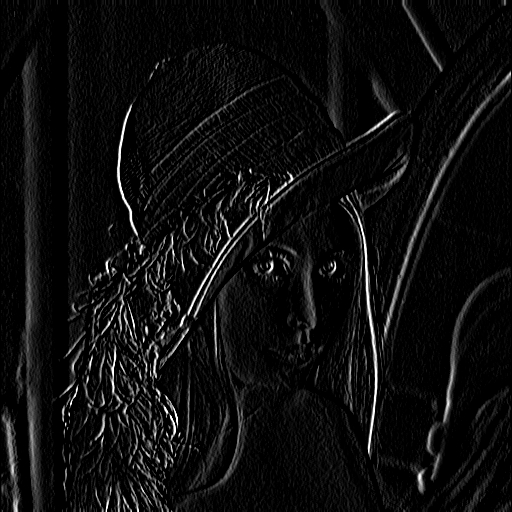
\includegraphics[width=0.3\textwidth]{kirs2-2}
	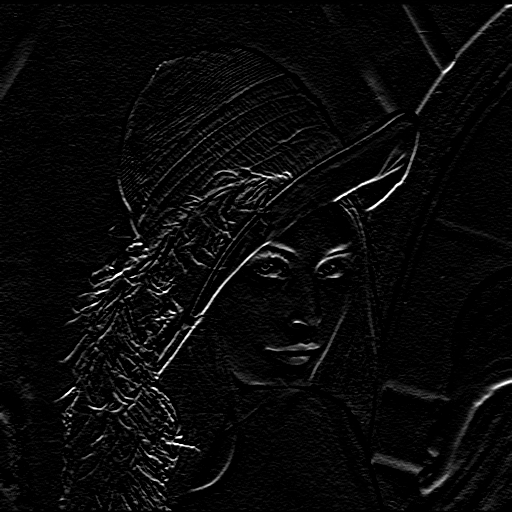
\includegraphics[width=0.3\textwidth]{kirs2-3}
	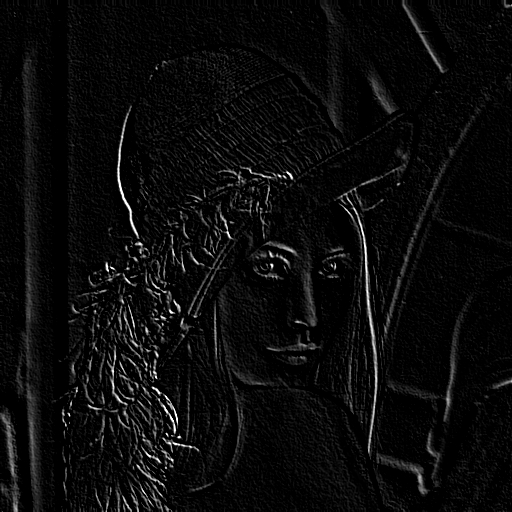
\includegraphics[width=0.3\textwidth]{kirs2-4}
	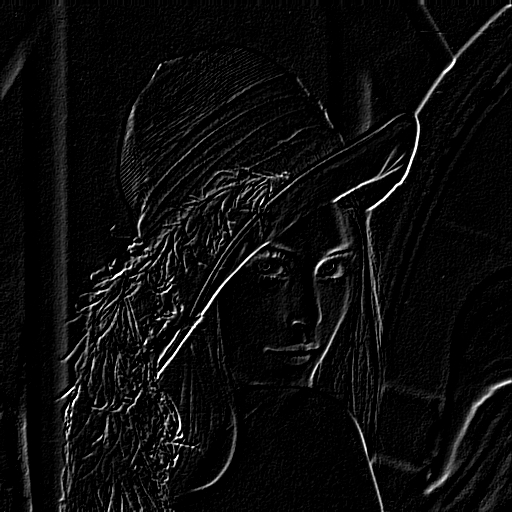
\includegraphics[width=0.3\textwidth]{kirs2-5}
	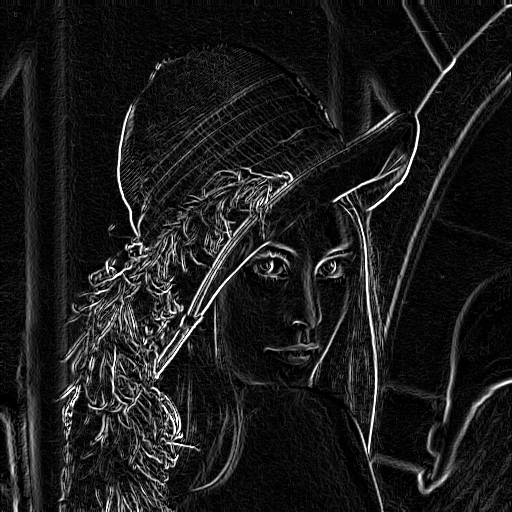
\includegraphics[width=0.3\textwidth]{kirs2-6}
  \caption{Applying Kirsch's operator to Lena's image without any other modifications.}
  \label{fig:kirs2}
\end{figure}

\end{homeworkProblem}

%----------------------------------------------------------------------------------------
%	Laplacian operator
%----------------------------------------------------------------------------------------

% To have just one problem per page, simply put a \clearpage after each problem

\begin{homeworkProblem}[\Roman{homeworkProblemCounter}. Laplacian Operator]
In this section, I have implemented the Laplacian operator on discrete images. This operator creates a new matrix out of an image which can be shown as an image but it might be meaningless because we are mapping the resulting matrix to the visible area with pixel of maximum value of 255. Laplacian operation can be done using different filters but the operator used in ColonD Image Processing program is as follows:
\[
F1 =\begin{bmatrix}
    0 & 1 & 0 \\
    1 & -4 & 1 \\
    0 & 1 & 0 
\end{bmatrix}
\]

At the rest of this section, I will provide some examples of the Laplacian operator applied to different images. Figures \ref{fig:lap1}, \ref{fig:lap2} and \ref{fig:lap3} are depicting these examples.

\begin{figure}[h!]
  \centering
	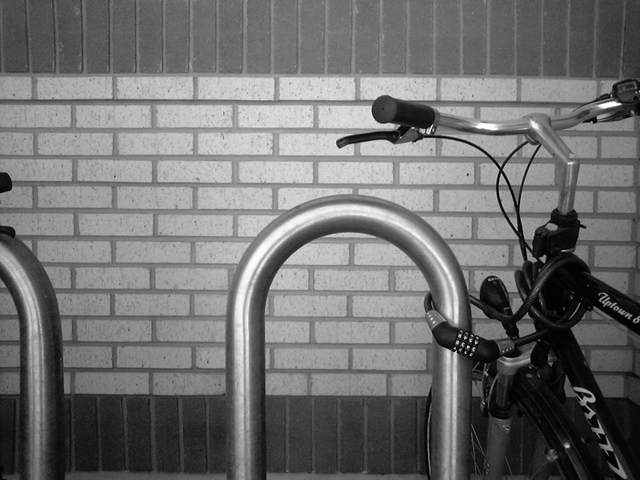
\includegraphics[width=0.3\textwidth]{lap1-1}
	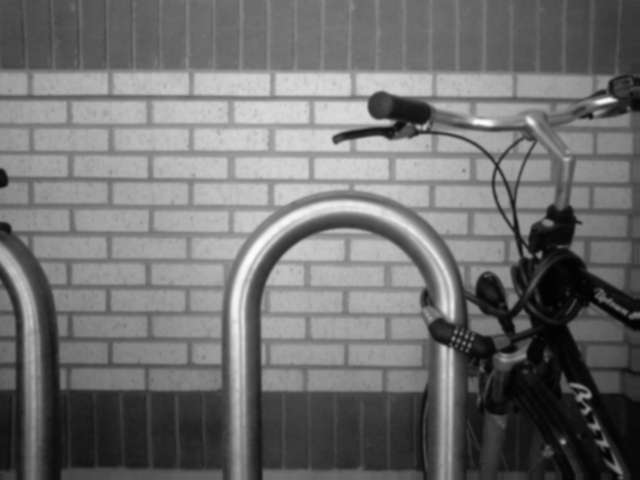
\includegraphics[width=0.3\textwidth]{lap1-2}
	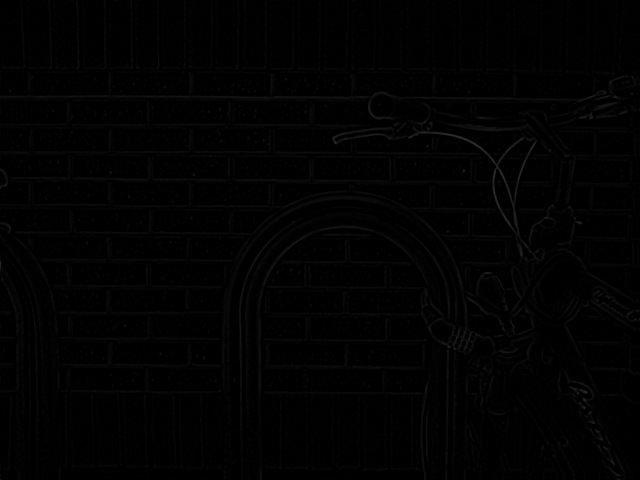
\includegraphics[width=0.3\textwidth]{lap1-3}
  \caption{Applying Guassian filter and Laplacian filter to the Bike's image.}
  \label{fig:lap1}
\end{figure}

\begin{figure}[h!]
  \centering
	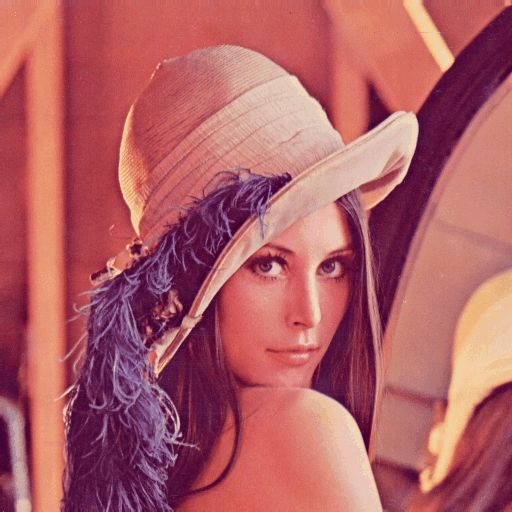
\includegraphics[width=0.3\textwidth]{lap2-1}
	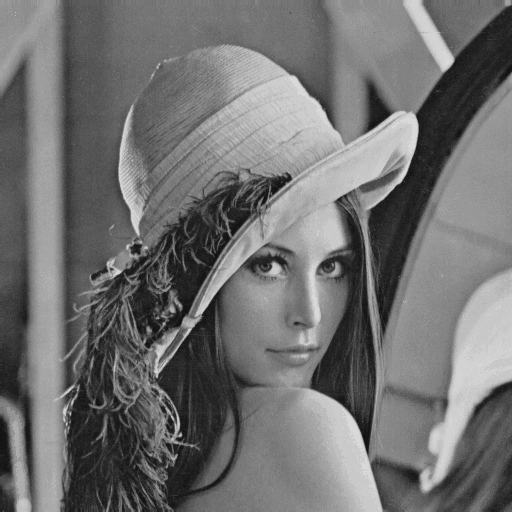
\includegraphics[width=0.3\textwidth]{lap2-2}
	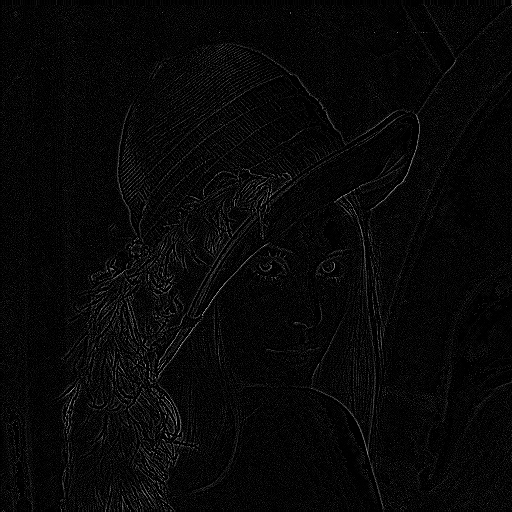
\includegraphics[width=0.3\textwidth]{lap2-3}
  \caption{Applying Gray-scale conversion and Laplacian filter to the Lena's image.}
  \label{fig:lap2}
\end{figure}

\begin{figure}[h!]
  \centering
	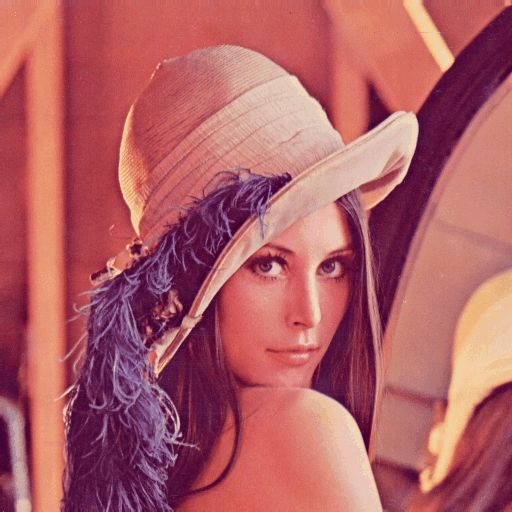
\includegraphics[width=0.3\textwidth]{lap3-1}
	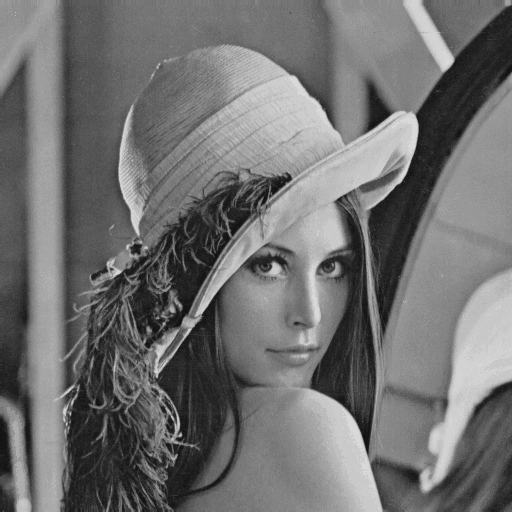
\includegraphics[width=0.3\textwidth]{lap3-2}
	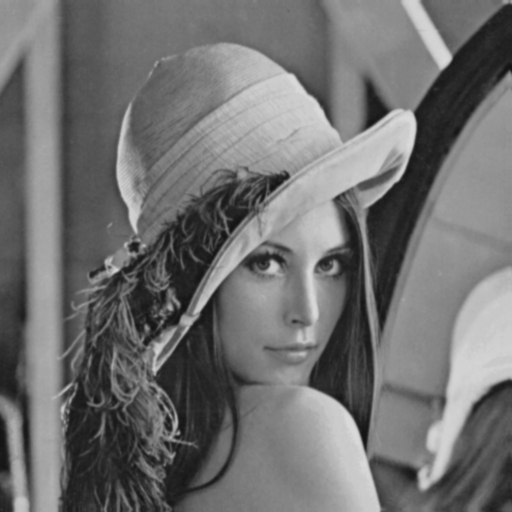
\includegraphics[width=0.3\textwidth]{lap3-3}
	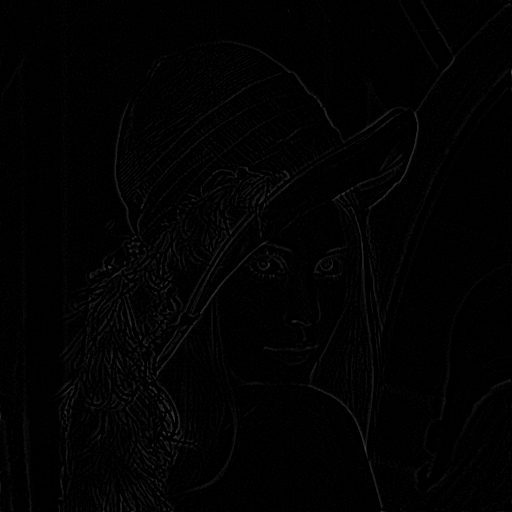
\includegraphics[width=0.3\textwidth]{lap3-4}
    \caption{Applying Gray-scale conversion, Guassian filter and Laplacian filter to the Lena's image. Applying just one step of the Guassian filter has a drastic effect on the result of the Laplacian operator. The highlighted areas get faded and less strong.}
  \label{fig:lap3}
\end{figure}

\end{homeworkProblem}

%----------------------------------------------------------------------------------------
%	Guassian operator
%----------------------------------------------------------------------------------------

% To have just one problem per page, simply put a \clearpage after each problem

\begin{homeworkProblem}[\Roman{homeworkProblemCounter}. Guassian Filter]
This is another Smoothing (low-pass) filter which is implemented in this program as an extra feature. Some examples of this filter applied once, twice and three times to one image is depicted in Figure \ref{fig:guas}.

\begin{figure}[h!]
  \centering
	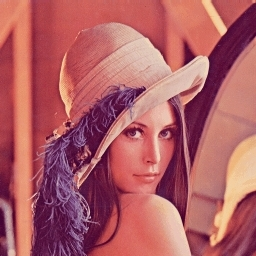
\includegraphics[width=0.3\textwidth]{guas1}
	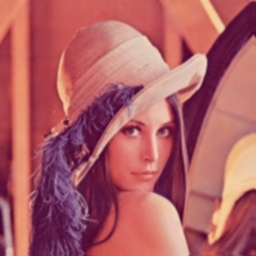
\includegraphics[width=0.3\textwidth]{guas2}
	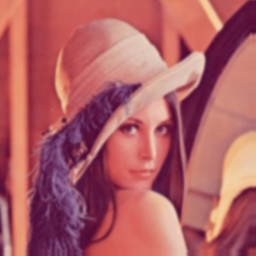
\includegraphics[width=0.3\textwidth]{guas3}
	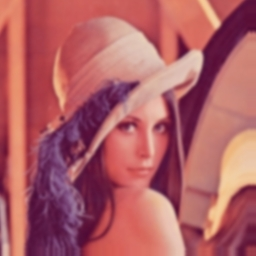
\includegraphics[width=0.3\textwidth]{guas4}
  \caption{Applying Guassian filter once, twice and three time to the Lena's image.}
  \label{fig:guas}
\end{figure}

\end{homeworkProblem}

%----------------------------------------------------------------------------------------
%	Conclusion
%----------------------------------------------------------------------------------------

% To have just one problem per page, simply put a \clearpage after each problem

\begin{homeworkProblem}[\Roman{homeworkProblemCounter}. Conclusion]
In this phase of the project, I implemented many high-pass filters which try to flatten out parts which have no significant changes in the pixel values but emphasize parts with rapid change in the pixel values.

\end{homeworkProblem}

\end{document}
